%%%%%%%%%%%%%%%%%%%%%%%%%%%%%%%%%%%%%%%%%%%%%%%%%%%%%%%%%%%%%%%%%%%%%%%%
% Plantilla TFG/TFM
% Escuela Politécnica Superior de la Universidad de Alicante
% Realizado por: Jose Manuel Requena Plens
% Contacto: info@jmrplens.com / Telegram:@jmrplens
%%%%%%%%%%%%%%%%%%%%%%%%%%%%%%%%%%%%%%%%%%%%%%%%%%%%%%%%%%%%%%%%%%%%%%%%

\chapter{Metodología}
\label{metodologia}
Una metodología de desarrollo de software es un marco de trabajo que se usa para estructurar, planificar y controlar el proceso de desarrollo de sistemas de información [\citep{def_metodologia}].

\section{Metodología de realización}
Para la  realización de este trabajo, se ha decidido utilizar la metodología SCRUM, basada en las siguientes aspectos [\cite{why_scrum}] :

\begin{itemize}
	\item \textbf{Adaptabilidad}: Los cambios pueden ser implementados en un proyecto en curso. Con Scrum puede variar lo que se debe hacer en un proyecto, pero el tiempo y coste son constantes.
	\item \textbf{Priorización de Tareas}: Las tareas se priorizan por orden de importancia, lo que generalmente significa que las tareas que se completan primero probablemente afectarán más al trabajo.
	\item \textbf{Sprints}: Los sprints son períodos delimitados durante el cual el equipo trabaja para completar una cantidad de trabajo [\cite{def_sprints}]. En nuestro caso, las planificación de los sprints se realizaba semanalmente, realizando un seguimiento a lo largo de la semana y presentando el incremento del trabajo al principio de la nueva reunión.
\end{itemize}

\section{Elección de las herramientas}
A continuación, detallamos las razones específicas para la elección de las siguientes herramientas como componentes clave del desarrollo.

\subsection{Github}

\begin{figure}[H]
    \centering
    
\includegraphics[width=6cm]{archivos/tfg_jorge/logos/github}
    \caption{Logo de Github}\label{sistemass2}
\end{figure}

Es una plataforma de online de desarrollo de software que nos facilitará el seguimiento de los cambios, pudiendo retroceder entre las nuevas versiones gracias a la tecnología en la que se basa Github, Git [\cite{def_github}].

Git es un software de control de versiones gratis y de código abierto, funciona como un rastreador de contenido permitiendo a los desarrolladores revertir y regresar a una versión anterior de su código. Con Git, cada desarrollador tiene una copia completa del repositorio, lo que permite trabajar sin conexión y realizar operaciones localmente. Además, Git soporta la creación de ramas para trabajar en nuevas características o correcciones de errores de manera independiente, que luego pueden fusionarse en la rama principal. Su uso de algoritmos de hashing garantiza la integridad de los datos, y su rendimiento superior permite manejar grandes cantidades de datos y cambios de manera eficiente [\cite{def_git}].

Por otro lado, Github ofrece un servicio para la gestión de proyectos, pudiendo definir listas de tareas dentro de un proyecto. Las listas de tareas que hemos considerado son las siguientes.

\begin{itemize}
	\item \textbf{Pendientes:} En esta lista se encuentran las tareas que se que no se han empezado a trabajar.
	\item \textbf{Proceso:} En esta lista se encuentran las tareas en las que se está trabajando en ese momento.
	\item \textbf{Bloqueadas:} En esta lista se encuentran las tareas que no pueden ser completadas debido a que dependen de otra que no se ha completado todavía.
	\item \textbf{Finalizadas:} En esta lista se encuentran las tareas que ya han sido completadas.
\end{itemize}

Los documentos compartidos y la planificación de reuniones se realiza mediante una aplicación de mensajería instantánea.

\subsection{Visual Studio Code}

\begin{figure}[H]
    \centering
    
\includegraphics[width=4cm]{archivos/tfg_jorge/logos/vscode}
    \caption{Logo de Visual Studio Code}\label{sistemass2}
\end{figure}

Un editor de código fuente desarrollado por Microsoft. Es un software libre y multiplataforma disponible para Windows, Linux y macOS. Tiene una buena integración con Git, incluyendo los comandos principales para las acciones en un repositorio remoto. Además, dispone de un gran número de extensiones para escribir y  ejecutar código en cualquier lenguaje de programación [\cite{def_vscode}].
Por todo esto hemos decidido que este entorno de programación es el más adecuado para llevar a cabo el trabajo.

\subsection{Draw.io}

\begin{figure}[H]
    \centering
    
\includegraphics[width=6cm]{archivos/tfg_jorge/logos/drawio}
    \caption{Logo de Draw.io}\label{sistemass2}
\end{figure}

Es una herramienta gratuita de diagramas en línea que permite a los usuarios crear una variedad de diagramas, gráficos y diagramas de flujo. Gracias a su interfaz intuitiva y su amplia gama de plantillas y figuras podremos dibujar cualquier diagrama para explicar cualquier estructura.

\subsection{Moqups}

\begin{figure}[H]
    \centering
    
\includegraphics[width=6cm]{archivos/tfg_jorge/logos/moqups}
    \caption{Logo de Moqups}\label{sistemass2}
\end{figure}

Esta herramienta online nos permitirá el diseño de prototipos para crear las interfaces de nuestra aplicación. Está diseñada para facilitar la colaboración en equipo y la visualización rápida de ideas de diseño. Algunas características clave para que podamos usarla incluyen su interfaz intuitiva y su biblioteca de componentes y plantillas, con componentes prediseñados, iconos y plantillas que podemos utilizar para acelerar el proceso de diseño.

\subsection{Vue.js}

\begin{figure}[H]
    \centering
    
\includegraphics[width=5cm]{archivos/tfg_jorge/logos/vuejs}
    \caption{Logo de Vue.js}\label{sistemass2}
\end{figure}

Es un framework progresivo para construir interfaces de usuario. Está diseñado desde cero para ser utilizado incrementalmente. La librería central está enfocada solo en la capa de visualización, y es fácil de utilizar e integrar con otras librerías o proyectos existentes [\cite{def_vue}].
Comparándolo con otros frameworks, podemos concluir que Vue.js es el más intuitivo para un usuario que empieza desde cero con los frameworks de desarrollo de interfaces, como Angular o React [\cite{comparar_vue}].


\subsubsection{Dependencias}
\subparagraph{Iconify}
%https://es.linux-console.net/?p=28105
%https://iconify.design/getting-started/

Iconify es un proyecto de código abierto que proporciona una forma sencillade utilizar iconos dentro de las aplicaciones Vue. El paquete que ofrece, \textbf{@iconify/vue}, permite agregar y personalizar rápidamente iconos en nuestro proyecto. Para instalarlo, ejecutaremos el comando de instalación:

\begin{lstlisting}[style=Consola, caption={Instalación del paquete iconify},label=Consola_code]
	npm install --save-dev @iconify/vue
\end{lstlisting}

Para agregar los iconos que ofrece Iconify debemos importar el componente Icon del paquete en nuestros componentes de Vue. Lo haremos con el siguiente fragmento de código:

\begin{lstlisting}[style=PHP-color, caption={Importar el componente Icon en Vue},label=PHP-color_code]
	<script setup>
		import { Icon } from '@iconify/vue'
	</script>
\end{lstlisting}

Para agregar iconos debemos buscar los que queramos en la página web de Iconify en [\citep{iconos-iconify}]. Una vez hayamos elegido el estilo del icono, podemos copiar el código del componente en la página web, por ejemplo:

\begin{lstlisting}[style=PHP-color, caption={Código para agregar un icono a la página},label=PHP-color_code]
	<template>
		<Icon icon="streamline:graph-dot-solid" />
	</template>
\end{lstlisting}

Dando como resultado:
\begin{figure}[H]
    \centering
    
\includegraphics[width=3cm]{archivos/tfg_jorge/icoco_grafico_iconify}
    \caption{Icono de gráfico importado desde la biblioteca de Iconify}\label{sistemass2}
\end{figure}

\subparagraph{ViteJS}
ViteJS es una herramienta de construcción de frontend que ofrece una experiencia de desarrollo moderna, rápida y eficiente para proyectos web.
Gracias a su recarga instantánea podemos mejorar considerablemente la productividad a medida que desarrollamos el proyecto. Nuestro proyecto principal de Vue lo crearemos con esta herramienta:

\begin{lstlisting}[style=Consola, caption={Instalación del paquete iconify},label=Consola_code]
	npm init @vitejs/app
\end{lstlisting}

\subparagraph{ChartJS}
Una biblioteca de JavaScript que permite crear gráficos interactivos y visualizaciones de datos en aplicaciones web. Es fácil de usar y compatible con múltiples tipos de gráficos, como barras, líneas, etc. Gracias a su sencillez para integrarla en nuestro proyecto de Vue podremos usarla con total normalidad.

Para usarla, crearemos un componente para la creación de una gráfica que podremos usar en todas las vistas que queramos:

\begin{lstlisting}[style=PHP-color, caption={Código para agregar un icono a la página},label=PHP-color_code]
<template>
  <div class="chart-container">
    <canvas :id="chartId"></canvas>
  </div>
</template>


<script>
import Chart from 'chart.js/auto';

export default {
  name: 'KpiChart',
  props: {
    chartData: {
      type: Array,
      required: true
    },
    chartId: {
      type: String,
      required: true
    },
    chartName: {
      type: String,
      required: true
    }
  },
  mounted() {

    try{
      const ctx = document.getElementById(this.chartId);
      if (this.chartData && this.chartData.length > 0) {
        new Chart(ctx, {
          type: 'line',
          data: {
            labels: this.chartData.map(row => row.time),
            datasets: [
              {
                label: this.chartName,
                data: this.chartData.map(row => row.score)
              }
            ]
          },
          options: {
            animation: {
              duration: 1500, // milisegundos
              easing: 'easeOutCubic', // Tipo de animación
              onProgress(animation) {
                const chartInstance = animation.chart;
                const ctx = chartInstance.ctx;
                const dataset = chartInstance.data.datasets[0];
                const meta = chartInstance.getDatasetMeta(0);
                meta.data.forEach((bar, index) => {
                  const data = dataset.data[index];
                  ctx.fillText(data, bar.x, bar.y - 5);
                });
              },
              onComplete(animation) {
                const chartInstance = animation.chart;
                const ctx = chartInstance.ctx;
                const dataset = chartInstance.data.datasets[0];
                const meta = chartInstance.getDatasetMeta(0);
                meta.data.forEach((bar, index) => {
                  const data = dataset.data[index];
                  ctx.fillText(data, bar.x, bar.y - 5);
                });
              }
            },
          }
        });
      } else {
        console.error('No hay datos para la grafica');
      }
    }
    catch(error){
      console.error("Error:",error)
    }
  }
};
</script>
\end{lstlisting}

Como resultado de una de nuestras gráficas:
\begin{figure}[H]
    \centering
    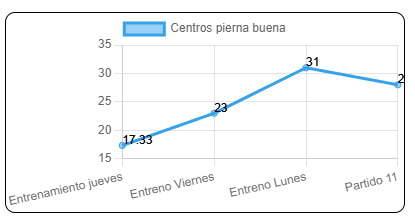
\includegraphics[width=10cm]{archivos/tfg_jorge/chartjs_ejemplo}
    \caption{Gráfico generado con ChartJS}
    \label{sistemass2}
\end{figure}

\subparagraph{Vue-router}
La biblioteca oficial de enrutamiento para Vue.js, diseñada para crear aplicaciones de una sola página (SPA). Proporciona una forma estructurada y eficiente de manejar las rutas y la navegación en una aplicación Vue.js [\cite{vue_route}]. Crear rutas para mostrar diferentes interfaces resultará muy sencillo añadiendo las rutas como la siguiente:

\begin{lstlisting}[style=PHP-color, caption={Código para agregar un icono a la página},label=PHP-color_code]
routes: [
  { path: '/user/:id', component: User }
]
\end{lstlisting}

\subparagraph{Vuex}
Sirve como un almacén centralizado para todos los componentes de una aplicación, con reglas que garantizan que el estado solo pueda ser mutado de manera predecible. Gracias a esto podremos crear variables globales que compartirán todos los componentes del proyecto de Vue.

\subsection{MySQL}

\begin{figure}[H]
    \centering
    
\includegraphics[width=5cm]{archivos/tfg_jorge/logos/mysql}
    \caption{Logo de MySQL}\label{sistemass2}
\end{figure}

Es el sistema de gestión de bases de datos relacional más extendido en la actualidad de código abierto que utiliza el lenguaje SQL (Structured Query Language) para acceder y gestionar datos almacenados en tablas. Siendo la elección popular para gestionar datos en entornos tanto pequeños como grandes, usaremos esta herramienta para la gestión de nuestra base de datos.

\subsection{Framework DAO}
Esta herramienta será proporcionada por el tutor Diego Marcos Jorquera. Se trata de un framework que gestiona los accesos a la base de datos, haciendo las peticiones desde la aplicación de Vue.js mucho mas sencillas. También ha sido implementado en los trabajos de [\cite{TFG_Sergio}] y [\cite{TFG_Daniel}].

